\documentclass{beamer}
\usepackage{graphicx}
\usepackage{booktabs}
\usepackage[scale=2]{ccicons}

\mode<presentation>
{
  \usetheme{Antibes}      % or try Darmstadt, Madrid, Warsaw, ...
  \usecolortheme{default} % or try albatross, beaver, crane, ...
  \usefonttheme{default}  % or try serif, structurebold, ...
  \setbeamertemplate{navigation symbols}{}
  \setbeamertemplate{caption}[numbered]
  \setbeamertemplate{footline}[frame number]
} 

\usepackage[utf8]{inputenc}
\usepackage[T1]{fontenc}
\usepackage[french]{babel}

\usepackage{natbib}

\title{Projet Transboost}
\author{Luc Blassel, Romain Gautron}
\date{22 Mars 2018}

\begin{document}

\begin{frame}
  \titlepage
\end{frame}

\section{Introduction}
\begin{frame}{Le projet Transboost}

\begin{itemize}
	\item Transfer learning $\rightarrow$ réutiliser des modèles entraînés
    \item boosting $\rightarrow$ faire des prédictions fortes a partir de plusieurs prédicteurs faibles
    \item associer les deux
\end{itemize}
    \medskip
    Succès dans la classification de séries temporelles incomplètes.\\
    Est-ce aussi efficace pour de la classification d'images avec des CNN?

\end{frame}

\section{Contexte}
\begin{frame}{Rappel sur le boosting}
	On part d'un ensemble de points pondérés:
    \begin{enumerate}
      \item on entraîne un classifieur faible
      \item on sur-pondère les points mal class\'es
      \item on sous-pondère les points bien class\'es
      \item on calcul le poids $\alpha_i$ du classifieur a partir de son erreur.
    \end{enumerate}
    \begin{block}{R\'esultat:}
      On fait la combinaison linéaire des $n$ classifieurs faibles pondérés avec les $\alpha_i$\\
      $\rightarrow$ on obtient un classifieur fort
    \end{block}
    
\end{frame}
\begin{frame}{Le principe derri\`ere Transboost}
	\begin{figure}
		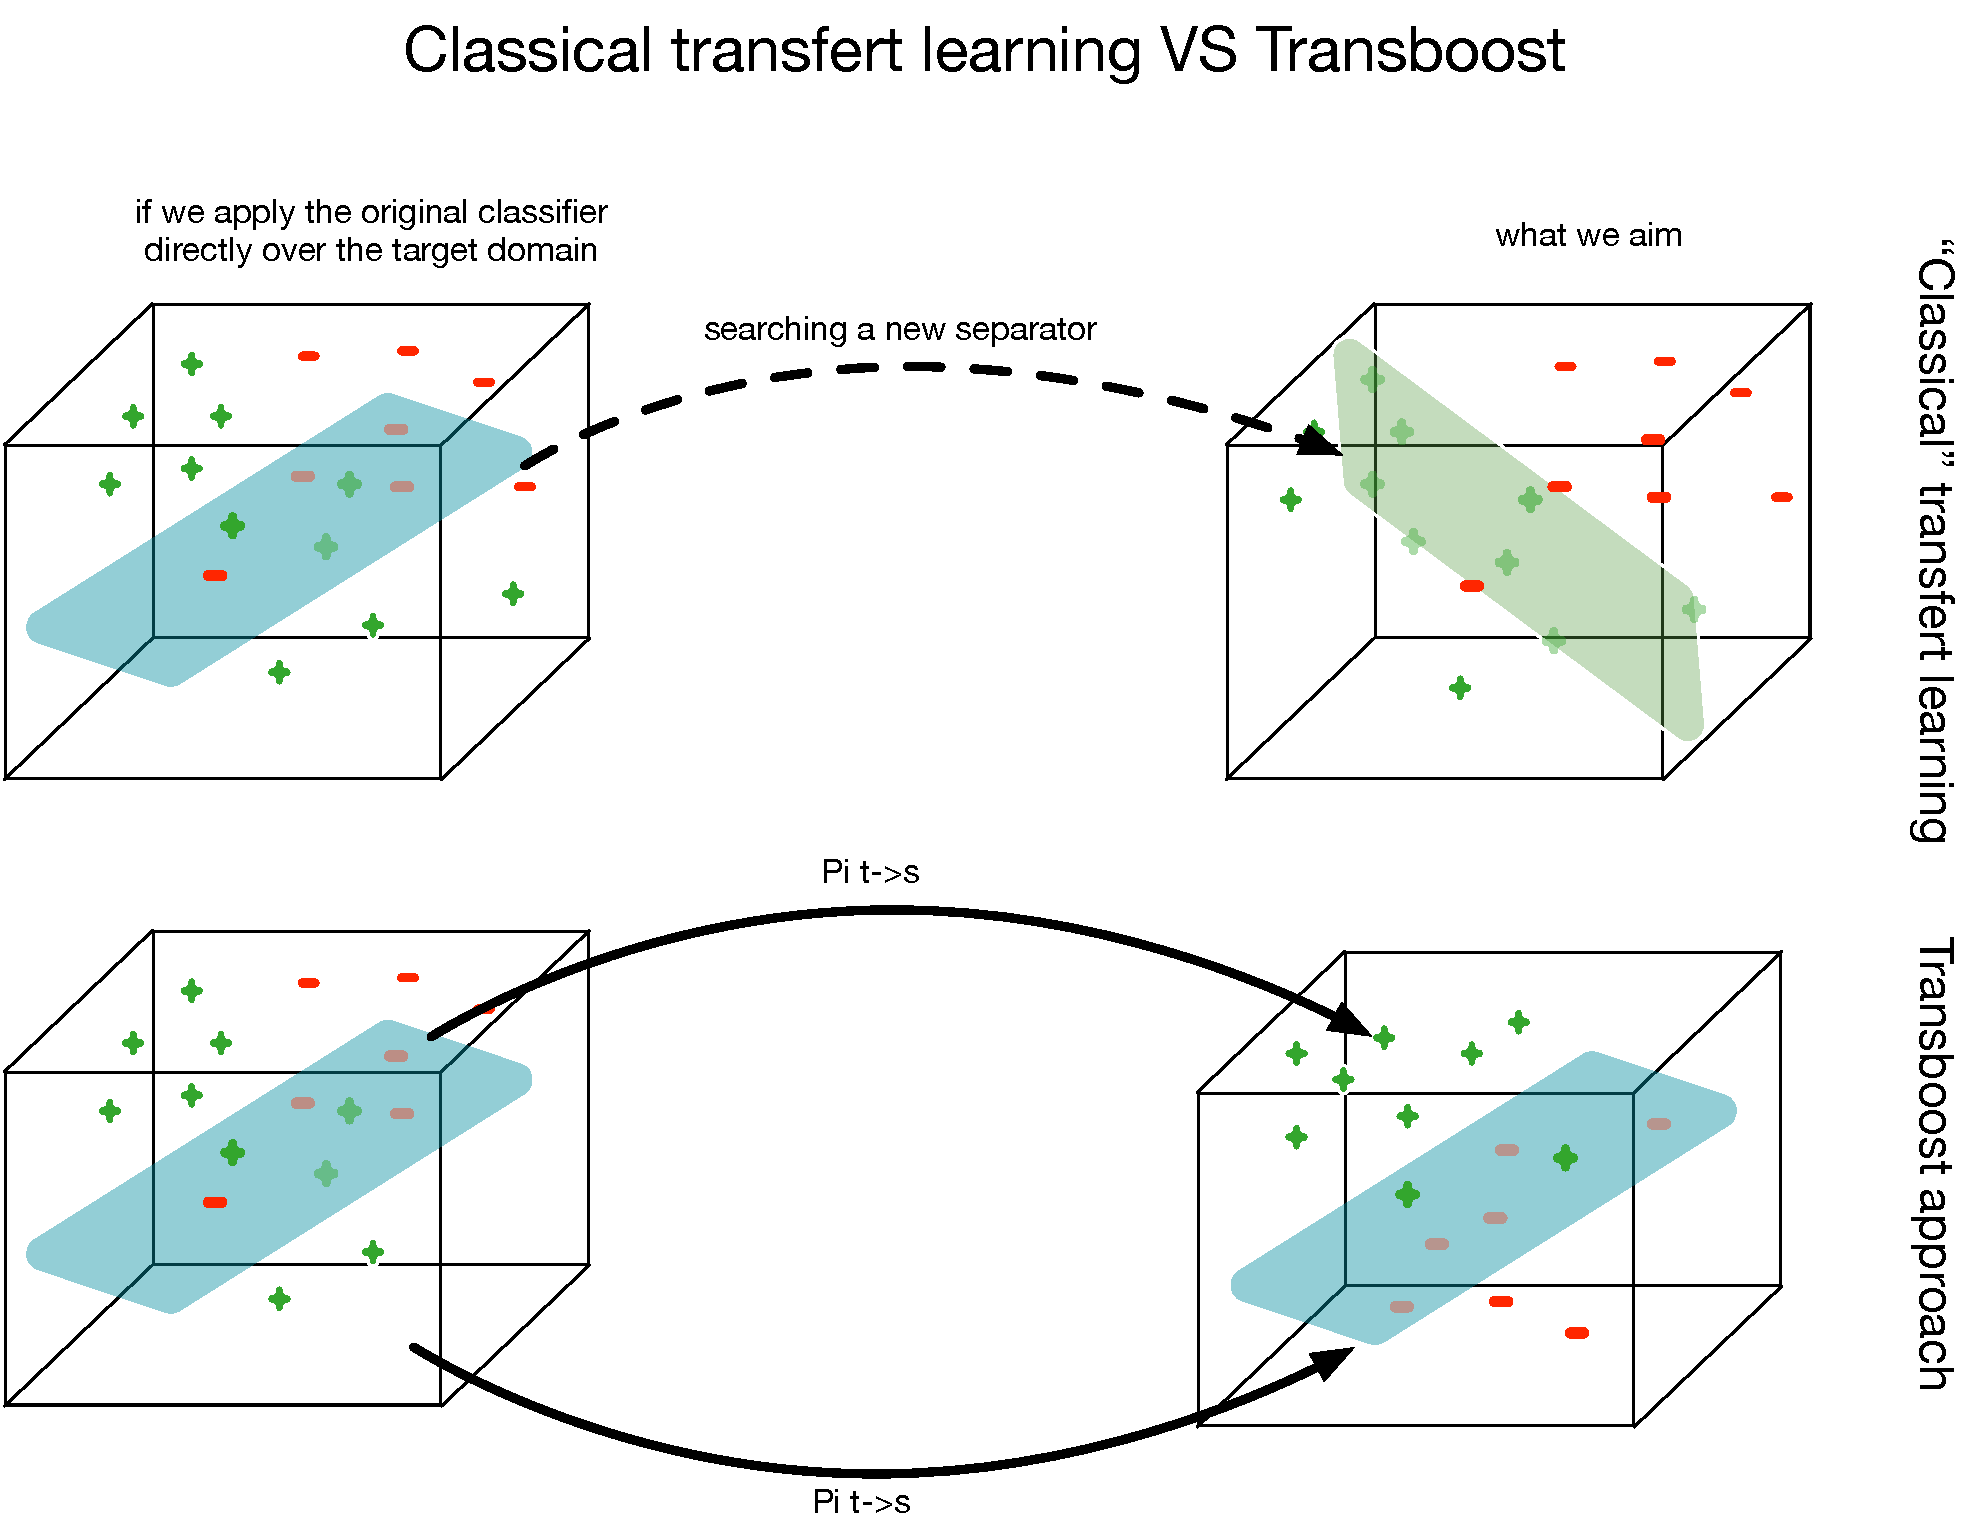
\includegraphics[width=.85\textwidth]{fig2.pdf}
	\end{figure}
\end{frame}

\begin{frame}{projection hamster $\rightarrow$ lion}
	\begin{figure}
		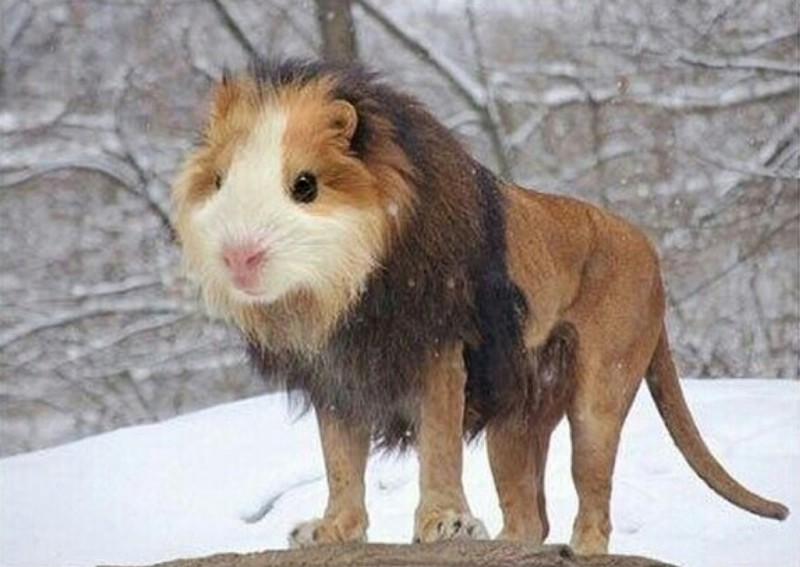
\includegraphics[width=.8\textwidth]{projectionImage.jpg}
	\end{figure}
\end{frame}
\section{Transboost avec des CNN: principe}
\begin{frame}{Transboost et réseaux de neurones}
	\begin{figure}
		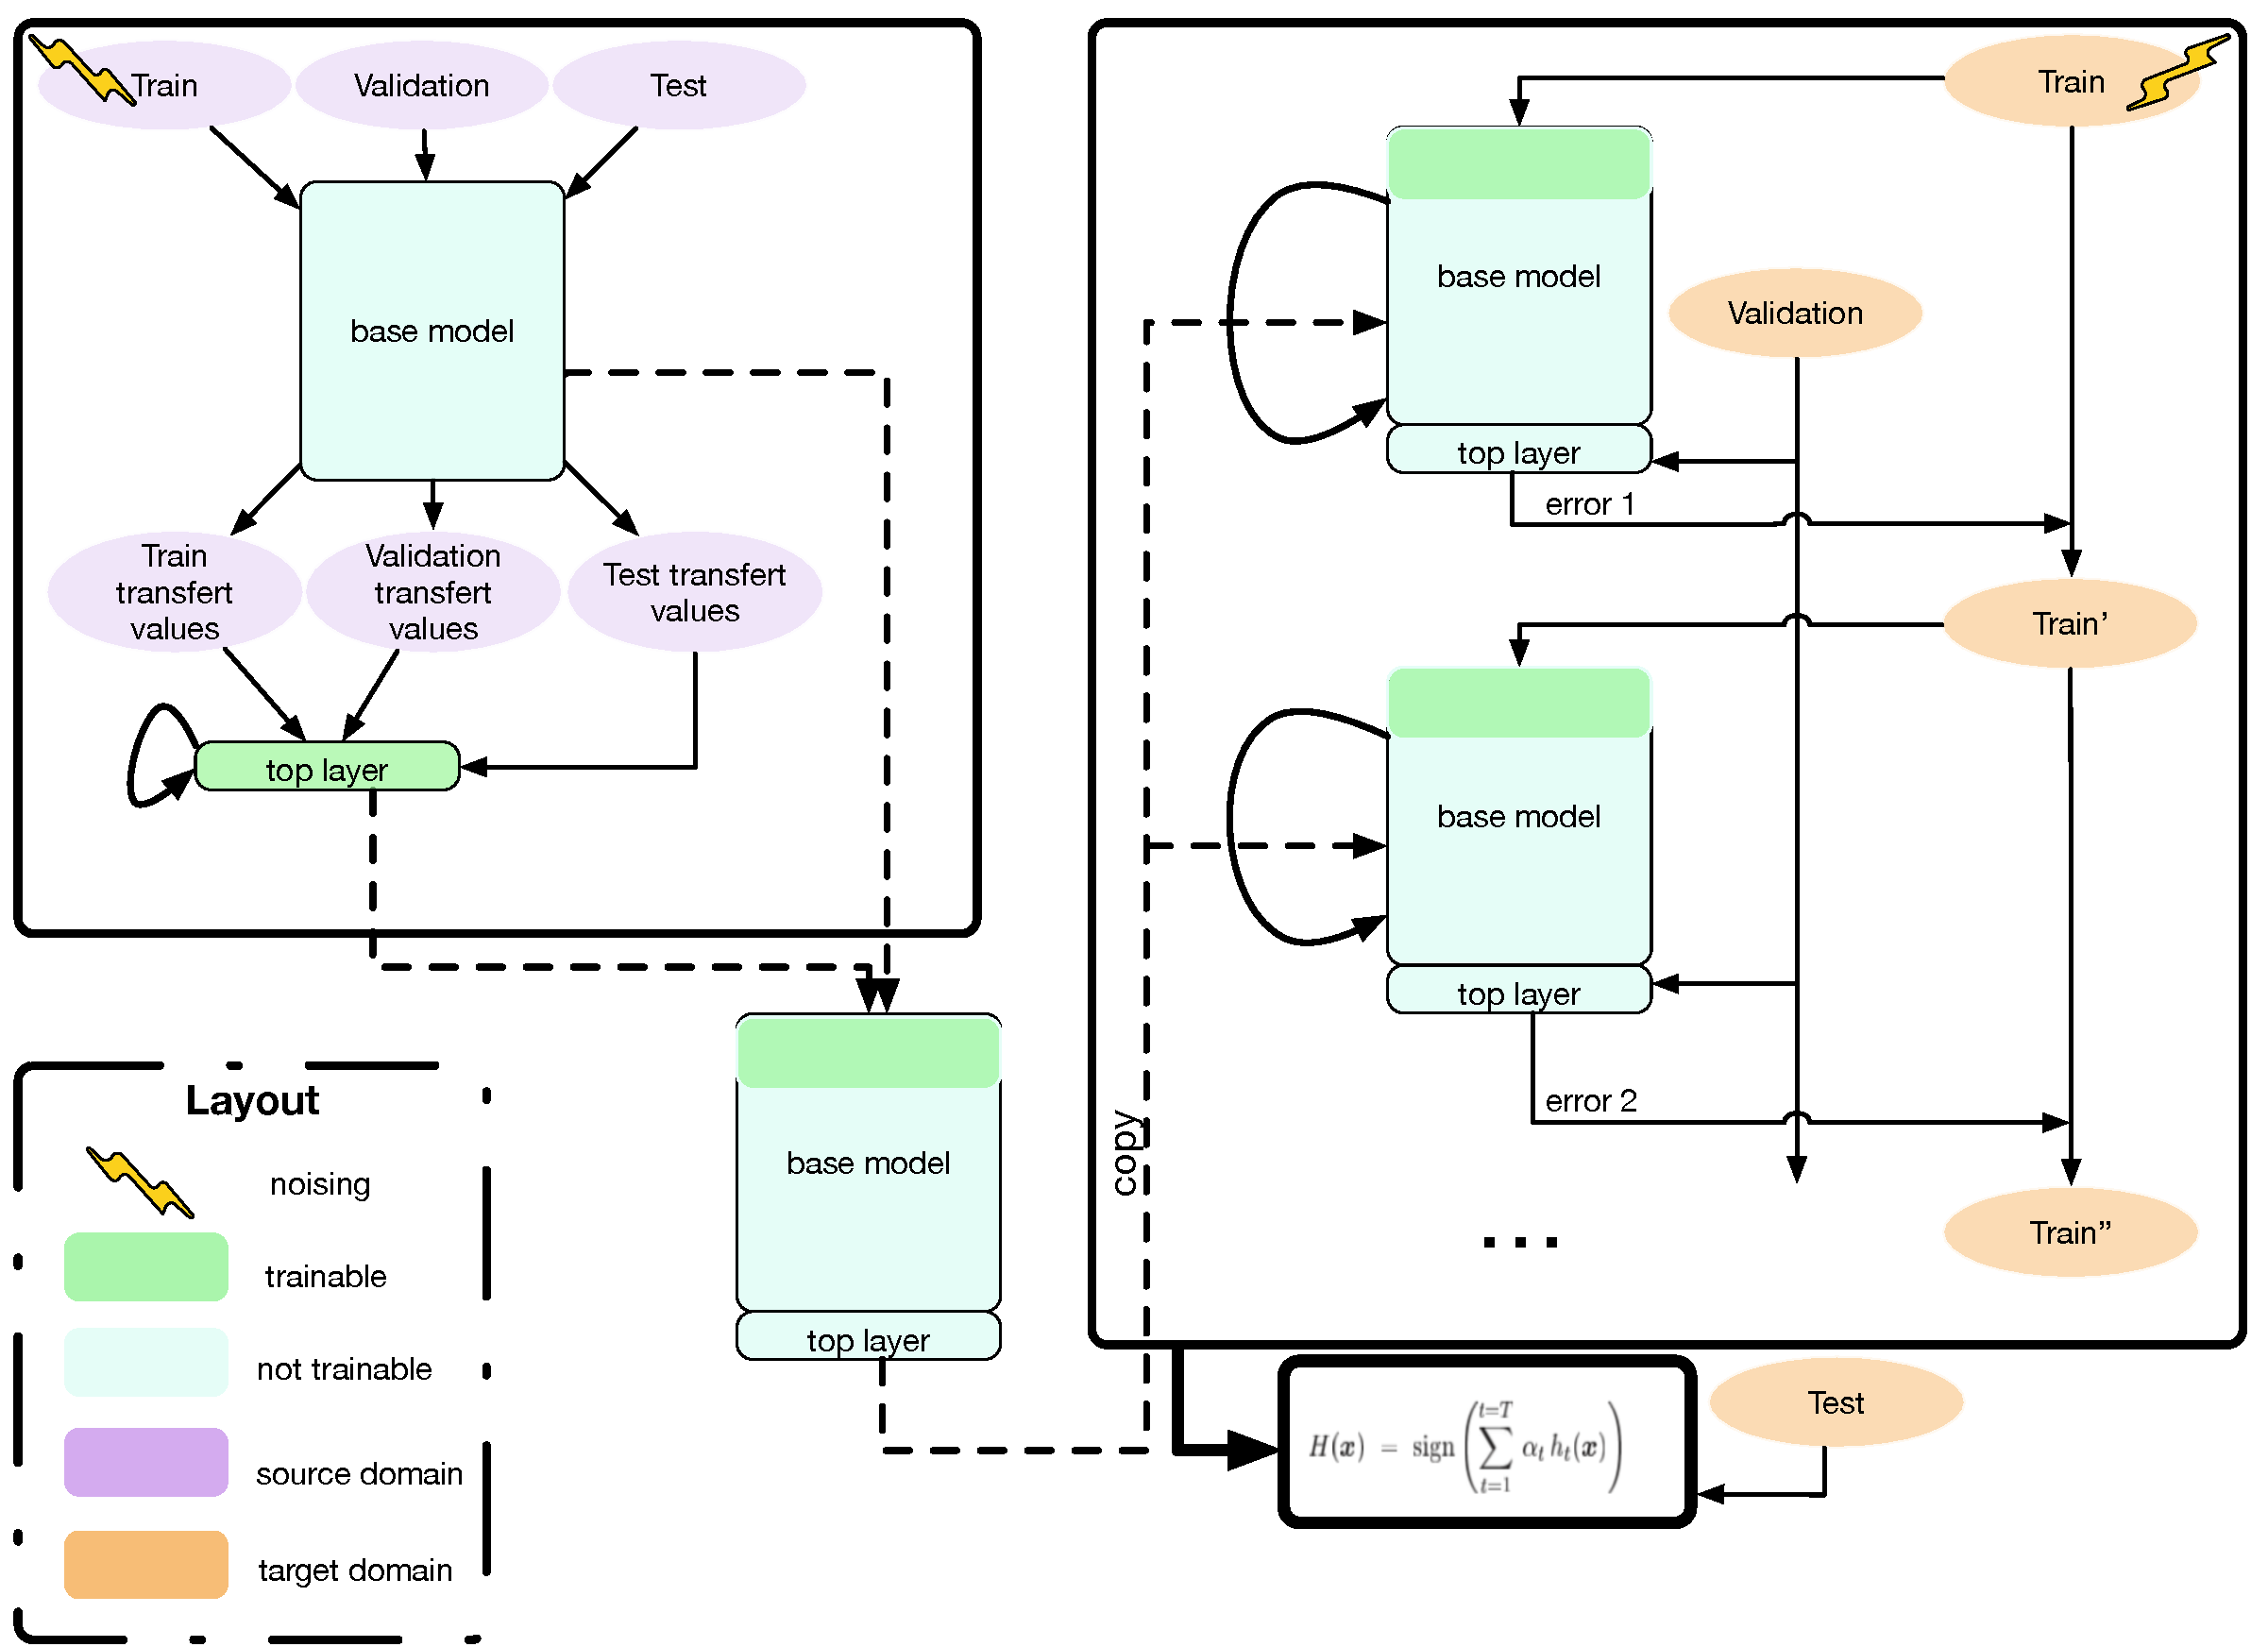
\includegraphics[width=.9\textwidth]{fig1.pdf}
	\end{figure}
\end{frame}

\section{Transboost avec des CNN: application}
	\subsection{Choix du dataset}
      \begin{frame}{CIFAR 10}
          \begin{figure}
          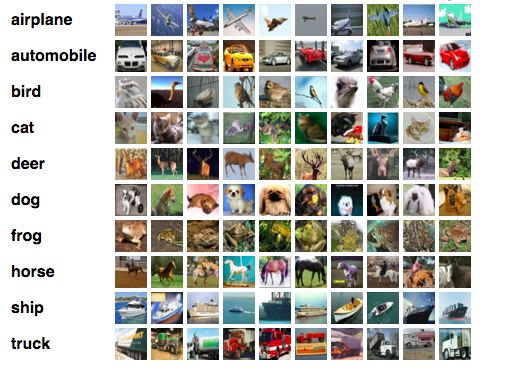
\includegraphics[width=.8\textheight]{cifar.png}
          \caption{CIFAR 10 dataset}
          \label{cifar1}
      \end{figure}
      \begin{itemize}
		\item 60 000 images : 50 000 train + 10 000 test
  	  \end{itemize}
    \end{frame}
    
    \subsection{Choix du modèle de base}
    \begin{frame}{Xception}
      \begin{figure}
          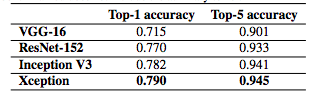
\includegraphics[width=.8\textheight]{xception.png}
          \caption{Comparaison des modèles de bases sur ImageNet}
          \label{cifar2}
      \begin{itemize} Sans fine tuning
      	\item 98.9 \% de précision sur dog/truck
        \item 92.2 \% sur deer/horse
      \end{itemize}
      \end{figure}
    \end{frame}
    
    \subsection{Conditions expérimentales}
    \begin{frame}{La machine}
      \begin{figure}
          
\includegraphics[width=.3\textwidth]{gcloud.png}
          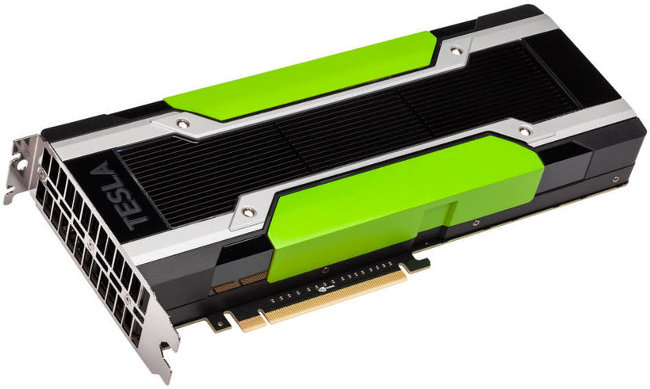
\includegraphics[width=.3\textwidth]{k80.jpg}
          
\includegraphics[width=.3\textwidth]{ubuntu.png}
          \caption{Setup}
          \label{Setup}
       \end{figure}
      \begin{itemize}
      	\item 8 coeurs
        \item 30 Go de RAM
        \item 12 Go de GPU
      \end{itemize}
    \end{frame}

    
    \subsection{Fonctionnement du programme}
    \begin{frame}{Fonctionnement du programme (1)}
      \begin{figure}
          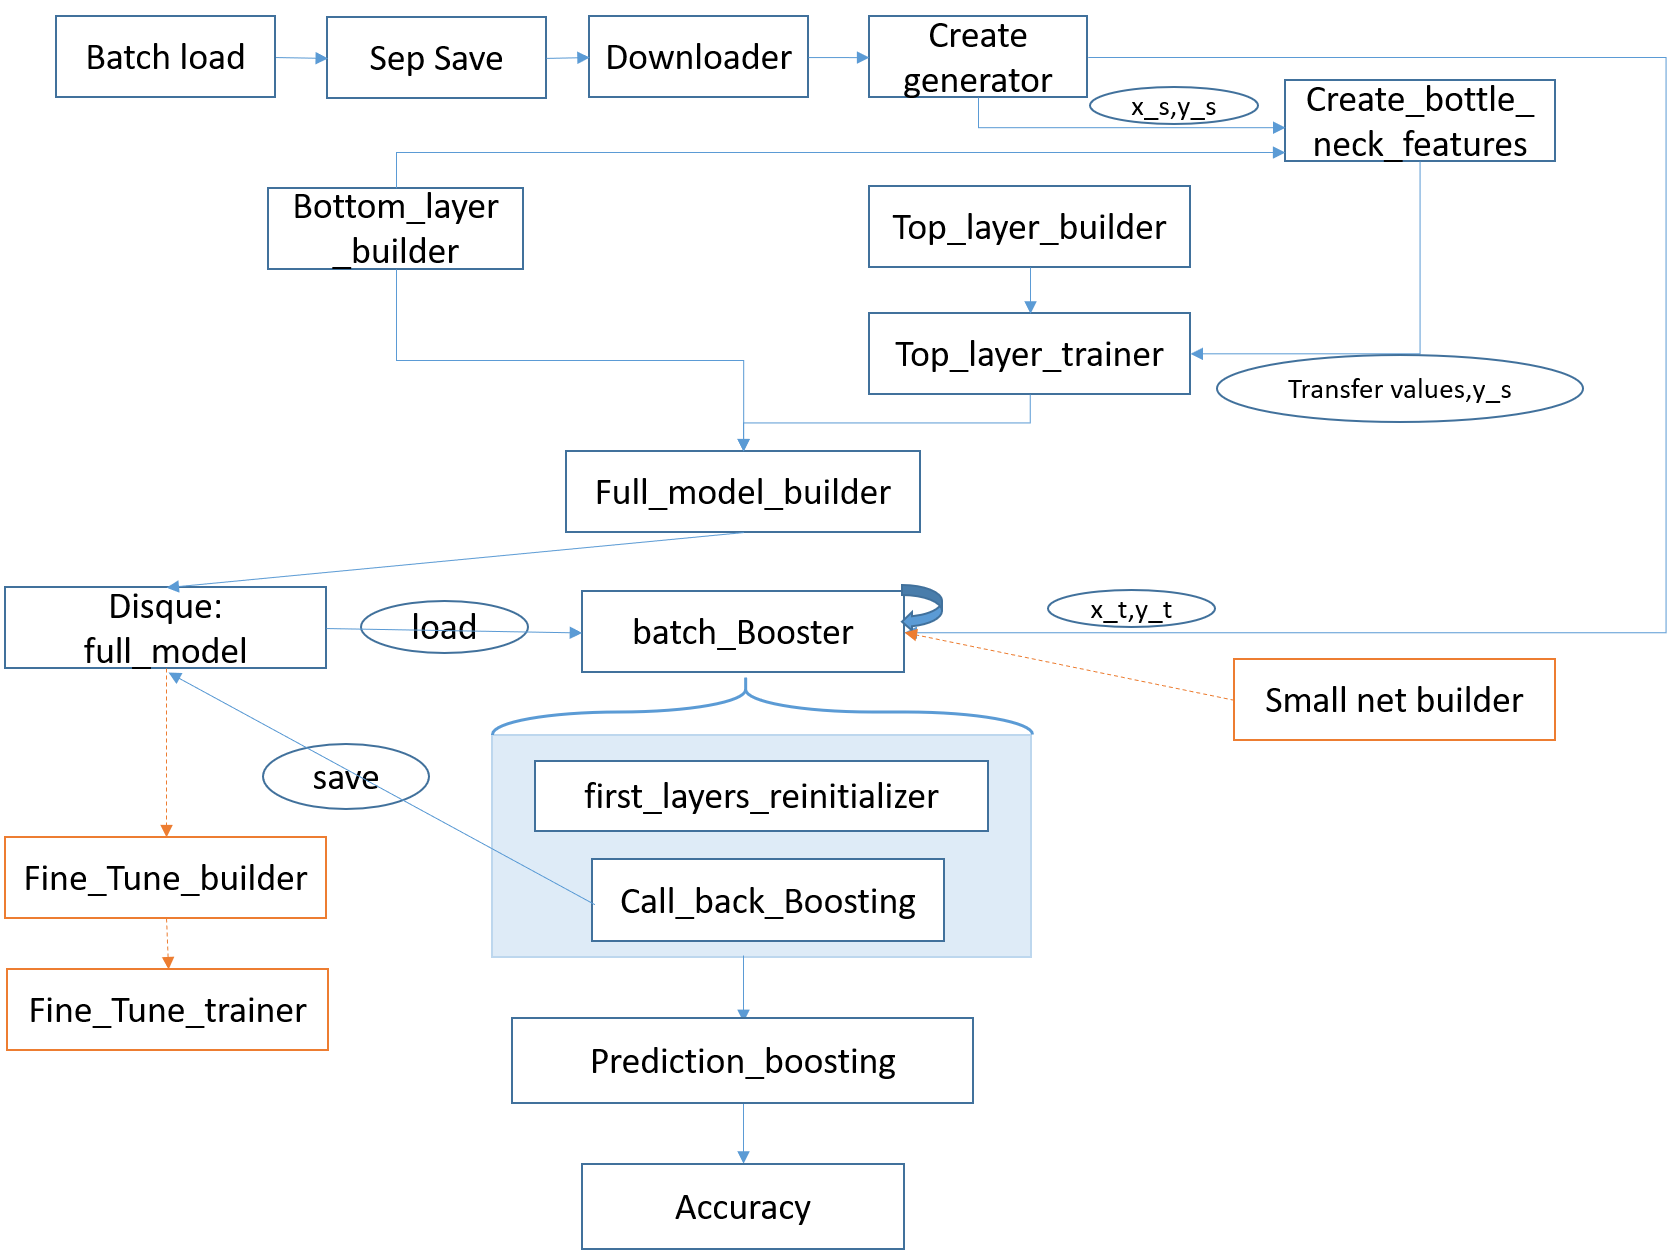
\includegraphics[height=.8\textheight]{programme.png}
          \caption{Programme}
          \label{Programme}
       \end{figure}
    \end{frame}
    
    \begin{frame}{Fonctionnement du programme (2)}
      \begin{figure}
          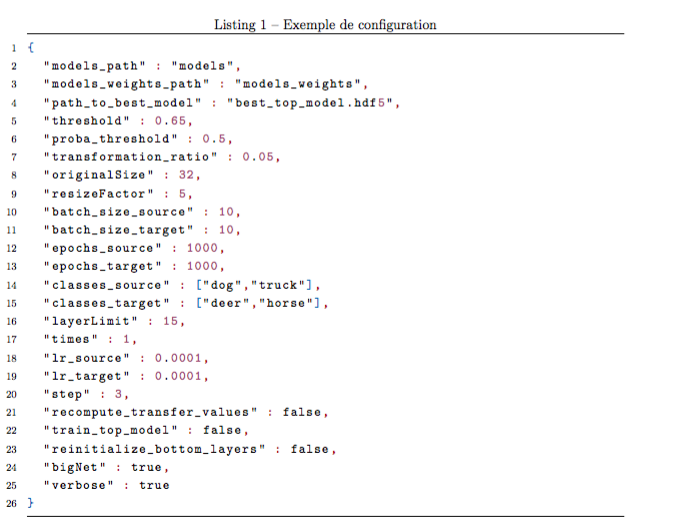
\includegraphics[width=.9\textheight]{config.png}
          \caption{Exemple de fichier de configuration}
          \label{Config}
       \end{figure}
    \end{frame}

\section{Expérimentations}
	\subsection{Boosting sur un petit CNN, pourquoi?}
    	\begin{frame}
         \begin{block}{Petit CNN} Apprentissage \`a partir de 0 directement sur le domaine cible dans le boosting
         $\rightarrow$ moins de back-propagation. 
         
         Nécessité d'utiliser un gros réseau ? 
         \end{block}
         
         \begin{figure}
         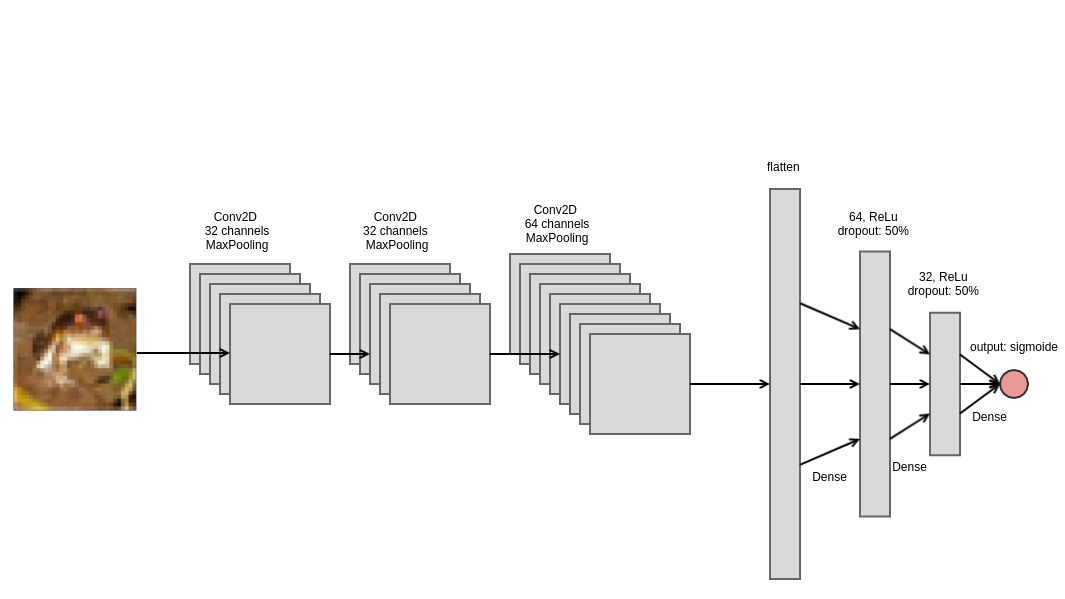
\includegraphics[width=.9\textwidth]{smallNetDraw.png}
         \end{figure}
     
    	\end{frame}
        
    \subsection{Résultat de petit CNN }
    	\begin{frame}
        
    		\begin{figure}[H]
            \begin{center}
            \centerline{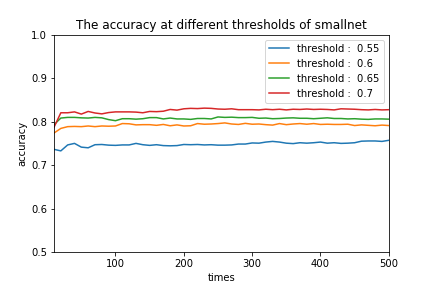
\includegraphics[width=0.7\textwidth]{smallnet.png}}
            \caption{Évolution de la précision de l'algorithme de Boosting avec des petits réseaux de convolution (sans transfert) }
            \label{fig:smallNet}
            \end{center}
            \end{figure}
        Plus le projecteur est fort, plus la précision augmente.  \newline
        L'algorithme de boosting a été correctement implémenté.  
        
    	\end{frame}
        
    \subsection{Résultats de Transboost}
    	\begin{frame}
%     	\begin{table}
%     	\begin{tabular}{c c c}
%       	\toprule
%        	seuil validation &résultat& temps de calcul \\
%         \midrule
% %       	0.55 & ne converge pas & 4h \\
% %       	0.60 & ne converge pas & 4h+ \\
%       	0.65 & ne converge pas & 4h+\\
%       	\bottomrule
%     \end{tabular}
%     \caption{Les résultats de différents seuils avec la méthode de Transboost}
%   	 \end{table}
%    Pour le seuil 0.65, on a obtient la précision 52\% sur l'ensemble de validation.\newline 
%    L'algorithme ne converge pas en un temps raisonnable quelque soit le seuil, on n'obtient que des projecteurs équivalents au hasard.

\begin{block}{Résultats de Transboost avec Xception}
Précision à chaque étape  de boosting .65 à 10 projecteurs $\rightarrow$ converge mais précision en test 51 \% environ

\bigskip

Premier projecteur : 52 \% environ sur le set de validation

\end{block}

\bigskip

$\hookrightarrow$ seuil .70 pour avoir au moins 55 \% de précision en validation ? Ne converge pas en 4h

\medskip

Divers configurations testées : classes, learning rate, optimiseur !!!

    	\end{frame}
    \subsection{Pas d’expériences sur les hyper-paramètres}
		\begin{frame}
        Influence des hyper-paramètres: recherche d'un optimum précision/coût calculatoire
        \begin{itemize}
        \item Influence de la force des projecteurs
        \item Influence du nombre de projecteurs
        \item Influence du nombre de blocs entraînés.\emph{(Dans l’idéal on veut en modifier le moins possible pour atteindre au plus vite le seuil de précision)}
        \end{itemize}
			
		\end{frame}
       
\section{Difficultés rencontrées}
    \subsection{De Tensor Flow à Keras}
	\begin{frame}
    \textbf{Tensor Flow}: compliquée à modifier la structure du modèle ou geler certaines couches.
    
    \textbf{Keras}: surcouche de Tensor Flow. Une syntaxe plus claire, des outils plus simples.
	\end{frame}
    
    \subsection{Performances limitées de machine}
	\begin{frame}
    Machines physiques/virtuelles : Temps d'exécution très long (dizaine d'heures et même en jours). Erreurs de mémoire.
	\end{frame}
    
    \subsection{gestion de la mémoire}
	\begin{frame}
    \begin{block}{probl\`emes de mémoire}
     Fonction $del$ de python ne garantit pas la suppression immédiate de l’objet.
    \end{block}
    
    Même en forçant l’exécution du \emph{"garbage collector"} du langage C (utilisé pour gérer la mémoire en Python), des modèles n'ont pas été entièrement supprimés.
    \newline
    
    $\Longrightarrow$ Perturbation de l’entraînement de nouveaux modèles.
    \end{frame}
    
	\begin{frame}
    \textbf{Solution:}
    
    \begin{itemize}
    
    \item Enregistrer les modèles (architecture et poids) sur le disque dur de la machine avec des fonctions de Keras.
    \item Utiliser la fonction $k.clear\_session()$ pour effacer tous les objets de la session.
    \item Créer un réseau chaque fois à partir de l’architecture sauvée et d’y charger les poids du modèle pour l'entraîner. 
    \end{itemize}
    \begin{block}{Inconvenient}
    temps d’accès beaucoup plus long du disque dur par rapport a la mémoire vive. \emph{(malgré tout très petit par rapport au temps d’entraînement)}
    \end{block}
    \end{frame}
    
\section{Conclusion}
	\begin{frame}
    \begin{itemize}
    	\item La méthode Transboost est séduisante sur les séries temporelles 
        \item Le boosting marche avec le petit CNN (sans transfert)
		\item Échec avec transfert \& gros CNN. Y a-t-il déstabilisation des couches de bas niveau?
        \item Challenge: Nécessité de capacité de calcul importante pour parcourir le réseau de convolution de base.
        \item le boosting pourrait peut-être marcher avec du transfer learning classique.
    \end{itemize}
	\end{frame}
    
\section*{sources}
	\begin{frame}{Bibliographie}
		\nocite*
        \bibliographystyle{plain}
        \bibliography{biblio.bib}
	\end{frame}

\end{document}
